\documentclass[12pt,a4paper]{article}
\usepackage[utf8]{inputenc}
\usepackage[T1]{fontenc}
\usepackage{geometry}
\geometry{margin=1in}
\usepackage{graphicx}
\usepackage{booktabs}
\usepackage{array}
\usepackage{amsmath}
\usepackage{hyperref}
\usepackage{cite}

\begin{document}

% -------------------- COVER PAGE --------------------
\begin{titlepage}
    \centering
    \vspace*{0.5cm}
    {\Large \textbf{VOICE-PIN SECURITY SYSTEM: SPOKEN DIGIT RECOGNITION AND SPEAKER VERIFICATION}\par}
    \vspace{1.2cm}

    {\itshape Submitted by\par}
    \vspace{0.3cm}
    {\large \textbf{Vanshika} (Reg. No: XXXXXXX)\par}
    {\large \textbf{Shreya} (Reg. No: XXXXXXX)\par}
    {\large \textbf{Kusum} (Reg. No: XXXXXXX)\par}
    \vspace{0.4cm}
    {\large \textbf{MSc AIML}\par}
    \vspace{0.2cm}
    {\large \textbf{Department of Computer Science}\par}
    \vspace{0.8cm}

    {\itshape for\par}
    \vspace{0.3cm}
    {\large \textbf{CONTINUOUS INTERNAL ASSESSMENT}\par}
    \vspace{0.6cm}

    {\itshape As part of\par}
    \vspace{0.3cm}
    {\large \textbf{MAI522-5}\par}
    {\Large \textbf{Speech Processing \& Recognition}\par}
    \vspace{1.0cm}

    \IfFileExists{CHRIST_Logo.jpg}{
        \includegraphics[width=2.4cm]{CHRIST_Logo.jpg}\par
    }{
        \vspace{2.4cm}
    }
    \vspace{0.8cm}

    {\large Department of Computer Science\par}
    {\large \textsc{Christ University Central Campus}\par}
    {\normalsize Bangalore, Karnataka, India -- 560029\par}
    \vspace{0.4cm}
    {\normalsize November 2026\par}
\end{titlepage}

% -------------------- TITLE & ABSTRACT --------------------
\setcounter{page}{1}
\begin{center}
    {\LARGE \textbf{Voice-PIN Security System: Spoken Digit Recognition and Speaker Verification}\par}
    \vspace{0.5cm}
    {\large November 25, 2026\par}
\end{center}

\begin{abstract}
This project implements a Voice-PIN unlock web application that recognizes spoken digits (\texttt{0}--\texttt{9}) and verifies the speaker's identity. For digit recognition, we compare Dynamic Time Warping (DTW), Gaussian Mixture Models (GMM), and Hidden Markov Models (HMM) using 39-dimensional Mel-Frequency Cepstral Coefficients (MFCCs with first and second derivatives). Audio is recorded in the browser using an \texttt{AudioWorklet} with decibel-based Voice Activity Detection (VAD) and sent to a FastAPI backend for silence trimming and classification. To reject non-digit words and background noise, the system checks both the confidence margin between the top two digits and a per-digit score threshold. We also add two-factor speaker verification using a Gaussian Mixture Model with a Universal Background Model (GMM-UBM) adapted via Maximum A Posteriori (MAP) estimation and Cepstral Mean and Variance Normalization (CMVN). On 55 test recordings from two speakers, \texttt{hmmlearn} HMM and our custom GMM both achieved \textbf{96.36\%} accuracy (53/55), multi-template DTW achieved \textbf{90.91\%} (50/55), and the speaker verifier separated the enrolled owner from an impostor.
\end{abstract}

% -------------------- 1. INTRODUCTION --------------------
\section{Introduction}
Voice-based PIN entry allows users to unlock an application hands-free by speaking a sequence of digits. In Speech Processing and Recognition (SPR), isolated-word recognition typically extracts spectral features such as MFCCs and classifies them with Dynamic Time Warping (DTW), Gaussian Mixture Models (GMMs), or Hidden Markov Models (HMMs)~\cite{rabiner1989tutorial}.

Moving from an offline script to a live microphone demo brings three main challenges:
\begin{enumerate}
    \item \textbf{Voice Activity Detection:} Live audio contains room noise, pauses, and soft starting sounds such as the /f/ in ``four''. A good endpoint detector needs pre-roll buffering and silence trimming so words are not cut off.
    \item \textbf{Noise and Unknown Words:} Standard classifiers always pick the closest digit among \texttt{0}--\texttt{9}, even if the user says a non-digit word or coughs. Score and margin checks are needed to reject unclear inputs.
    \item \textbf{Speaker Identity:} Digit recognition alone only checks what was said, not who said it. Adding speaker verification ensures that another person cannot unlock the app even if they know the PIN.
\end{enumerate}
To handle these points, we built a web interface where users can record their own digit samples, retrain all models with one click, and test live PIN unlocking with optional speaker verification.

% -------------------- 2. RELATED WORKS --------------------
\section{Related Works}
Early isolated-word recognition systems used Dynamic Time Warping (DTW) to align speech sequences of different lengths~\cite{sakoe1978dynamic}. Davis and Mermelstein~\cite{davis1980comparison} showed that MFCCs capture vocal-tract characteristics better than linear filterbank energies. Rabiner~\cite{rabiner1989tutorial} popularized HMMs for modeling the time order of speech sounds across states. For speaker verification, Reynolds et al.~\cite{reynolds2000speaker} introduced the GMM-UBM approach, where a shared Universal Background Model is adapted to a target speaker using MAP adaptation. Table~\ref{tab:related_works} lists these reference methods.

\begin{table}[h!]
\centering
\caption{Summary of foundational methods in isolated-word recognition and speaker verification.}
\label{tab:related_works}
\small
\begin{tabular}{p{2.4cm} p{2.3cm} p{2.6cm} p{2.5cm} p{3.2cm}}
\toprule
\textbf{Task} & \textbf{Features} & \textbf{Preprocessing} & \textbf{Model} & \textbf{Reference \& Year} \\
\midrule
Isolated Word Alignment & Spectral / Cepstral Frames & Endpoint Detection & Dynamic Time Warping (DTW) & Sakoe \& Chiba~\cite{sakoe1978dynamic}, 1978 \\
Feature Extraction & Mel-Filterbank Cepstra & Pre-emphasis, Hamming Window & MFCC (13 + $\Delta$ + $\Delta\Delta$) & Davis \& Mermelstein~\cite{davis1980comparison}, 1980 \\
Isolated Digit Recognition & MFCC Sequences & Dual-threshold Energy + ZCR & Hidden Markov Model (HMM) & Rabiner~\cite{rabiner1989tutorial}, 1989 \\
Speaker Verification & Cepstral Vectors & CMVN, Silence Removal & GMM-UBM with MAP Adaptation & Reynolds et al.~\cite{reynolds2000speaker}, 2000 \\
\bottomrule
\end{tabular}
\end{table}

% -------------------- 3. PROJECT OBJECTIVES --------------------
\section{Project Objectives}
\begin{itemize}
    \item To fix and compare five isolated-digit (\texttt{0}--\texttt{9}) classifiers (DTW, custom GMM, \texttt{scikit-learn} GMM, custom HMM, and \texttt{hmmlearn} HMM) using 39-dimensional MFCC features.
    \item To build a browser-based Voice-PIN demo with live VAD, silence trimming, rejection of unclear audio, and built-in voice recording for multi-speaker enrollment.
    \item To add two-factor speaker verification using a CMVN-normalized GMM-UBM so the system checks both the spoken PIN and the speaker's voice.
\end{itemize}

\subsection{Proposed Methodology}
Training recordings and live unlock attempts go through the same audio pipeline:
\begin{enumerate}
    \item \textbf{Browser Capture and VAD:} An \texttt{AudioWorklet} reads microphone audio in the browser. It estimates the room noise level in decibels during a $0.5\text{ s}$ calibration step and updates it during silence. Speech recording starts when the signal rises $8\text{ dB}$ above the noise floor for $60\text{ ms}$, keeping $200\text{ ms}$ of pre-roll audio and waiting $350\text{ ms}$ of silence before stopping.
    \item \textbf{Trimming and MFCC Extraction:} The FastAPI backend resamples each WAV clip to $22{,}050\text{ Hz}$, trims silence using \texttt{librosa.effects.trim} (\texttt{top\_db=25}), checks that the duration is between $0.16\text{ s}$ and $1.25\text{ s}$, normalizes peak amplitude, and computes 39 MFCC features ($13$ static, $13\ \Delta$, $13\ \Delta\Delta$).
    \item \textbf{Digit Classification and Rejection:} We store up to 8 templates per digit for multi-template DTW (accelerated with Numba) instead of averaging across speakers, train custom diagonal GMMs with \texttt{logsumexp} and variance flooring, and pass explicit utterance \texttt{lengths} to \texttt{hmmlearn}. A prediction is accepted only if it passes a minimum margin over the second-best digit and a 5th-percentile per-digit training score threshold.
    \item \textbf{Speaker Verification (GMM-UBM):} A 24-component diagonal UBM is trained on background speakers using utterance-level CMVN (to reduce microphone differences between laptops) and MAP-adapted ($\tau = 8.0$) to the enrolled owner. Across a 4-digit PIN, the average log-likelihood ratio $\text{LLR}(X) = \log P(X \mid \lambda_{\text{owner}}) - \log P(X \mid \lambda_{\text{UBM}})$ must meet the calibrated threshold.
\end{enumerate}

\begin{figure}[h!]
    \centering
    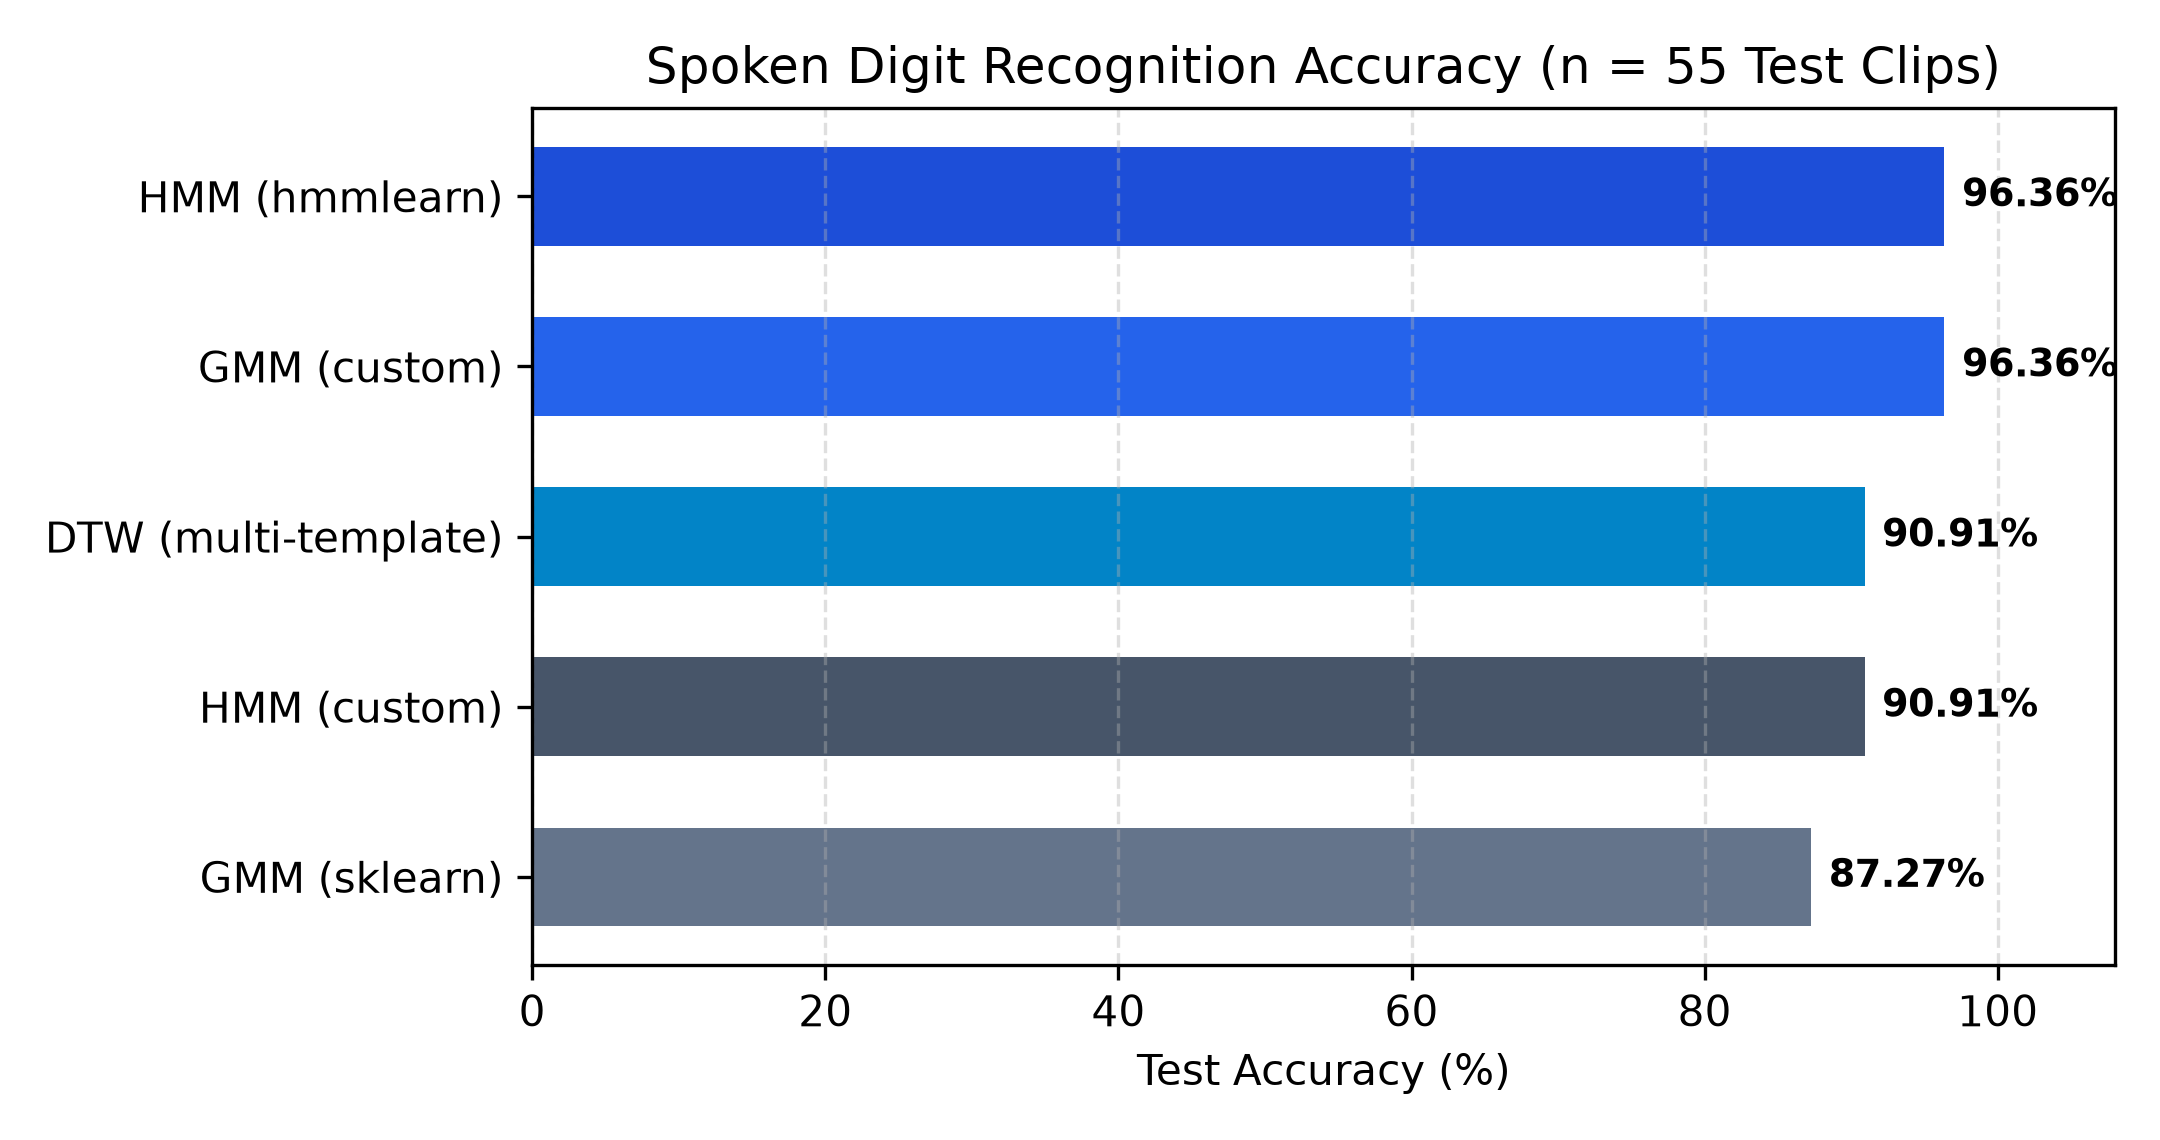
\includegraphics[width=0.84\textwidth]{Figures/model_accuracy.png}
    \caption{Test accuracy comparison across the five digit recognition models on the multi-speaker enrolled dataset (55 held-out test utterances).}
    \label{fig:model_comparison}
\end{figure}

\begin{figure}[h!]
    \centering
    \begin{minipage}{0.48\textwidth}
        \centering
        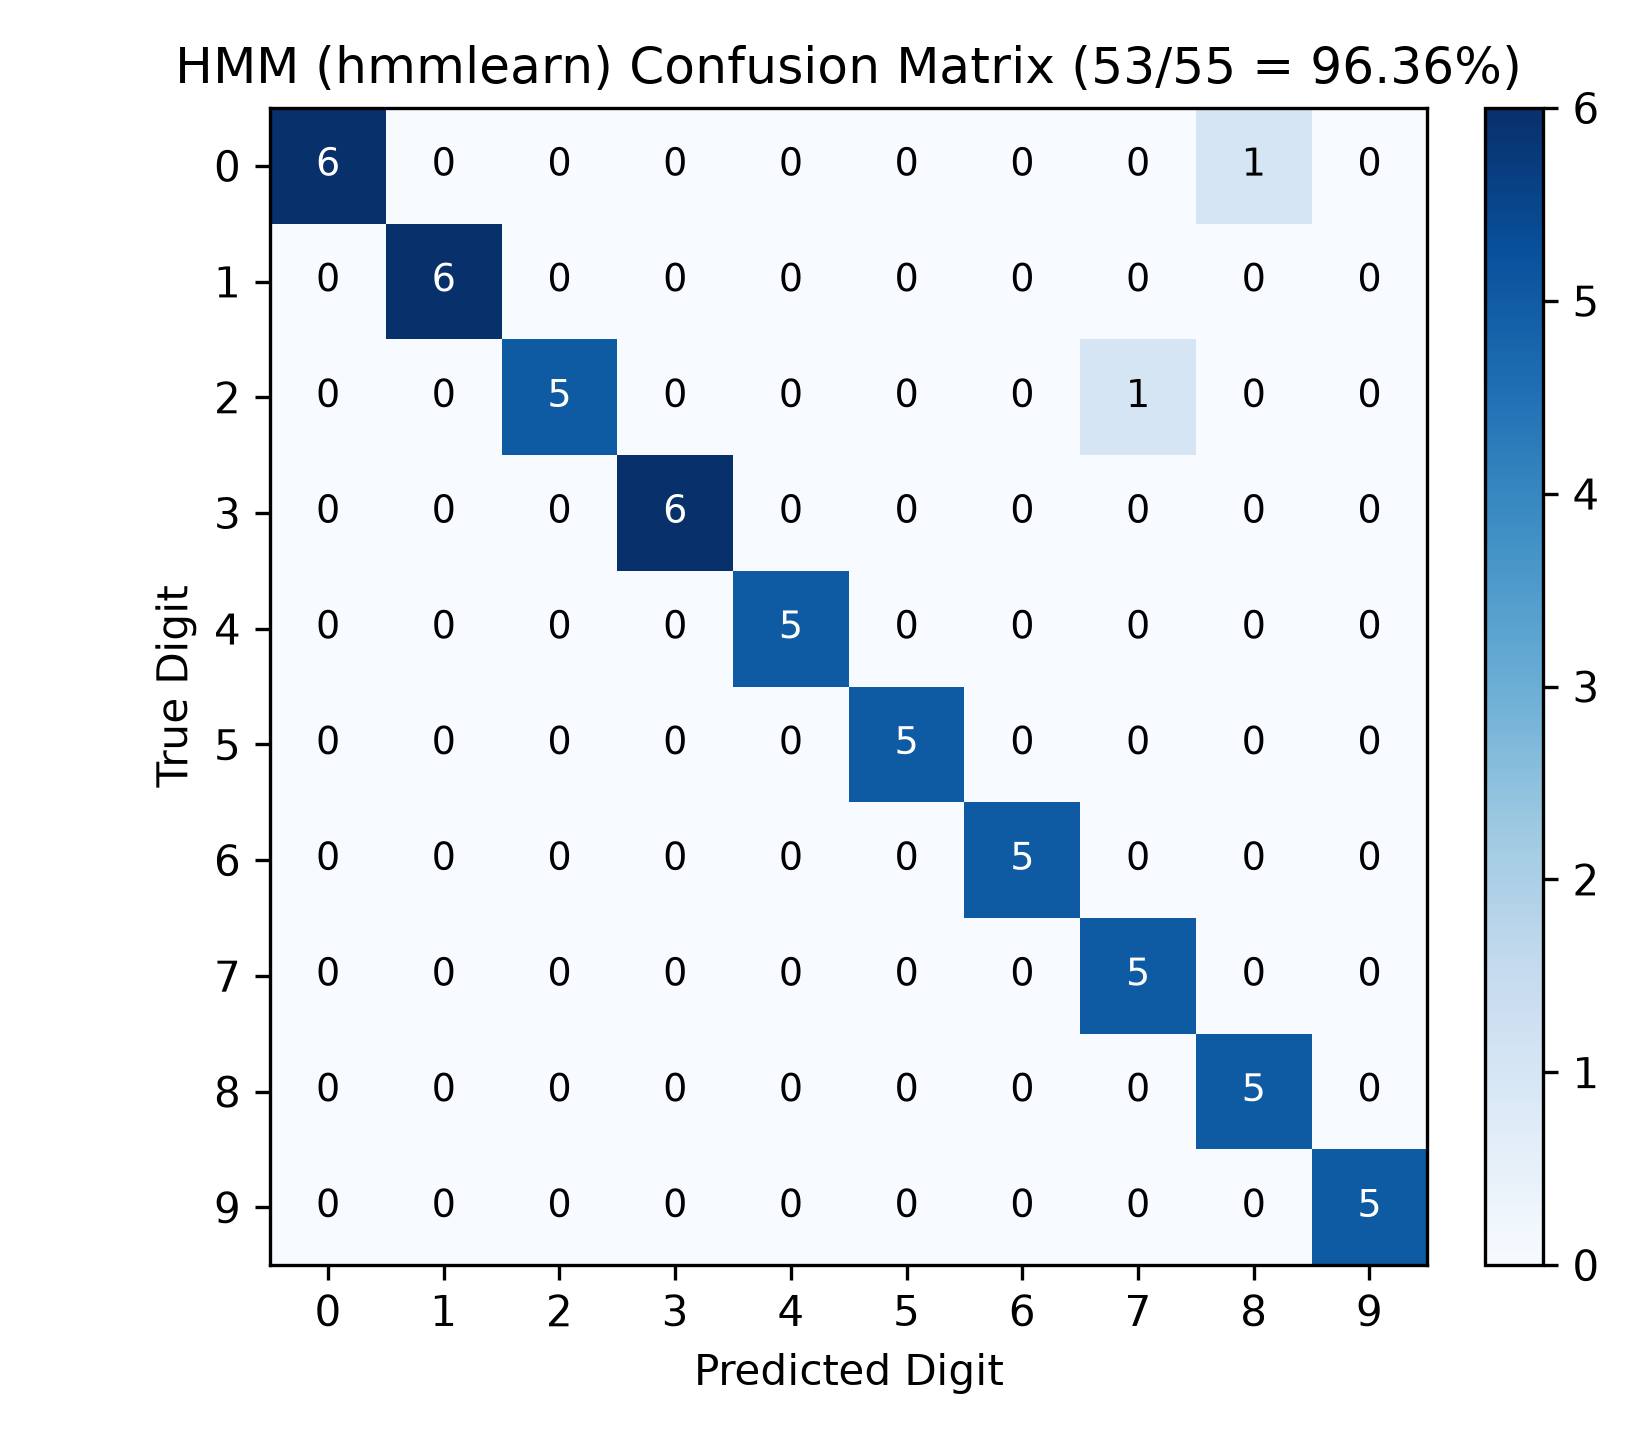
\includegraphics[width=\textwidth]{Figures/confusion_matrix.png}
        \caption{10$\times$10 confusion matrix of \texttt{hmmlearn} HMM on the 55 held-out test utterances.}
        \label{fig:confusion_matrix}
    \end{minipage}\hfill
    \begin{minipage}{0.49\textwidth}
        \centering
        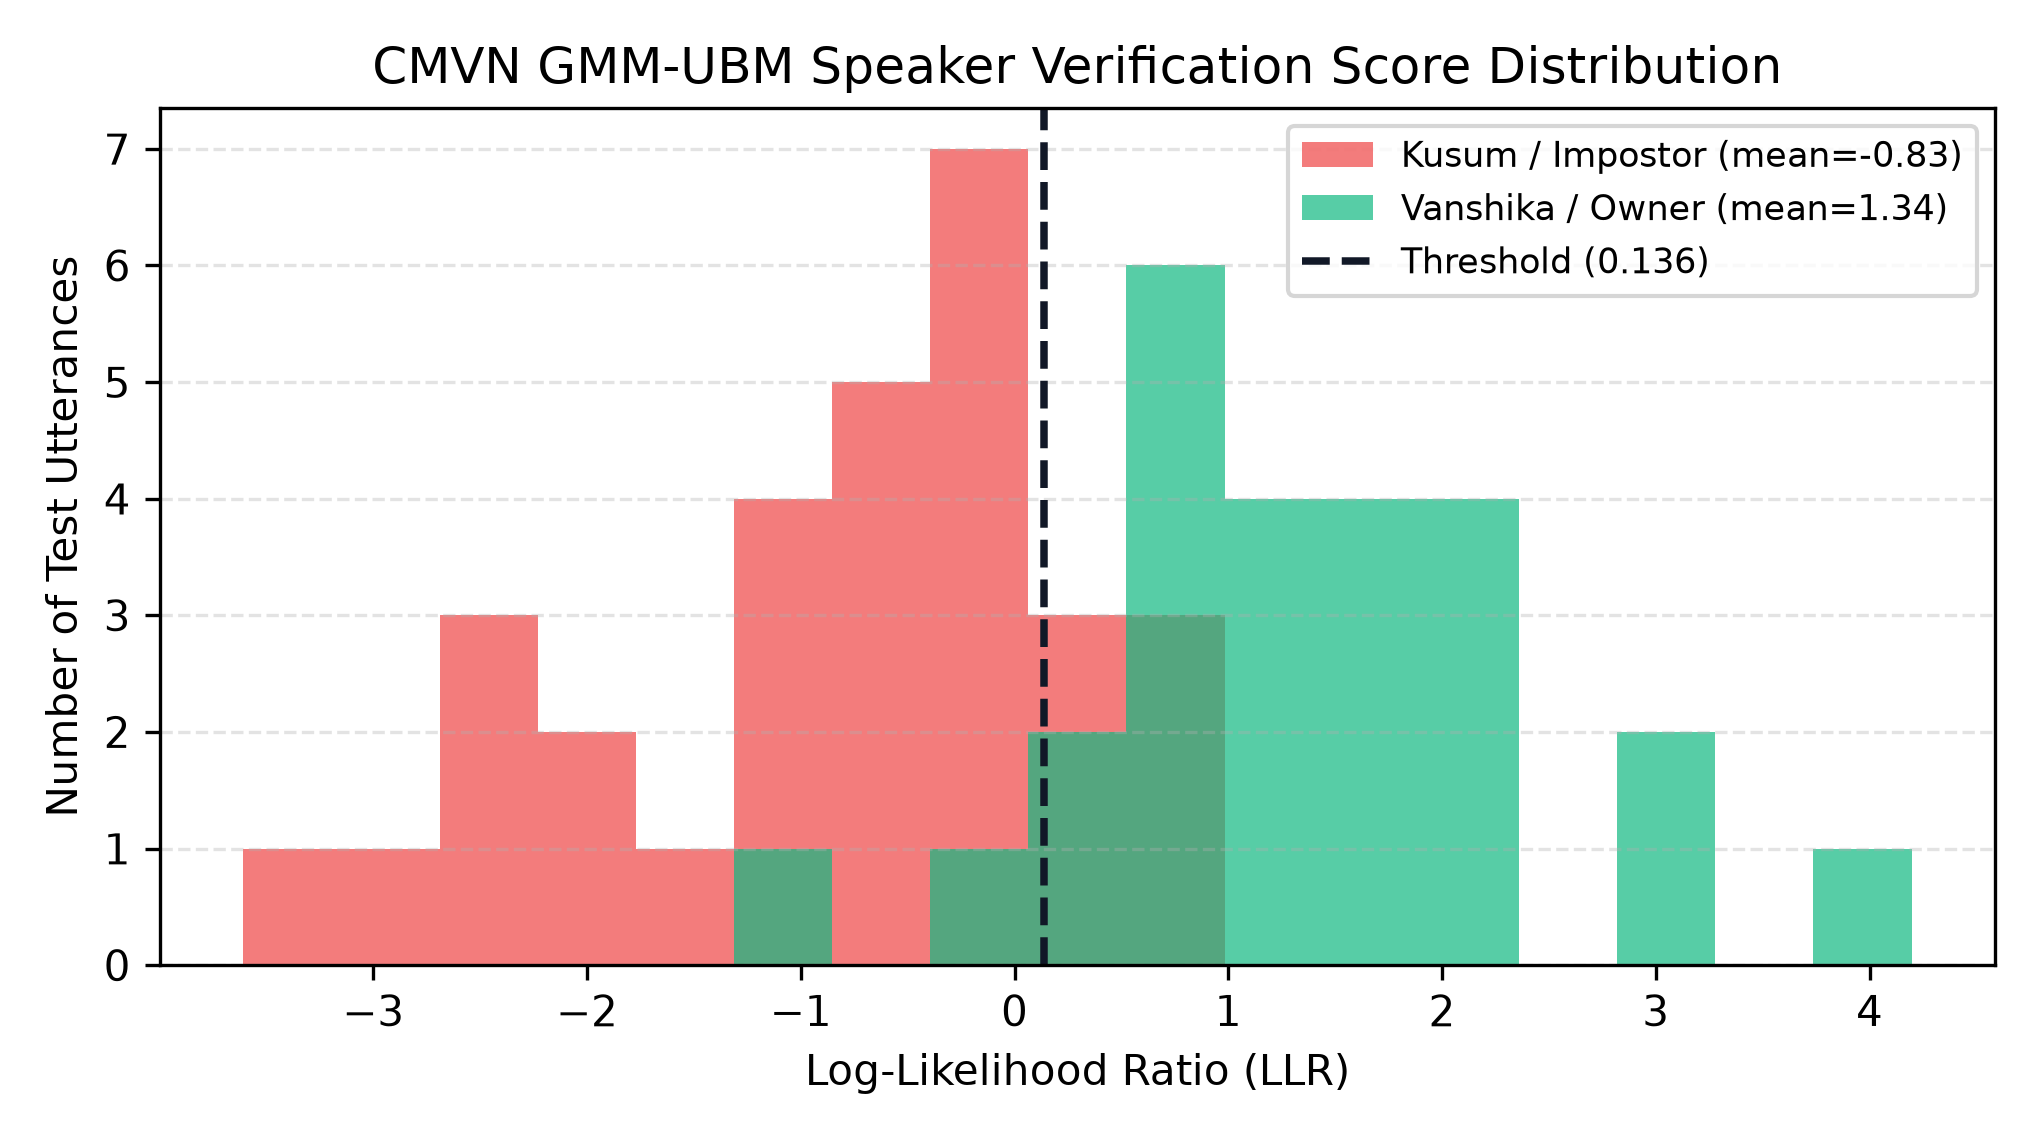
\includegraphics[width=\textwidth]{Figures/speaker_llr.png}
        \caption{CMVN GMM-UBM speaker verification LLR distribution (Owner vs.\ Impostor).}
        \label{fig:speaker_llr}
    \end{minipage}
\end{figure}

% -------------------- 4. CONCLUSIONS --------------------
\section{Conclusions}
In this project, we built a working Voice-PIN web application using classical SPR models. After fixing numerical issues (NumPy 2.0 compatibility, \texttt{logsumexp} scoring, variance flooring, sequence lengths in \texttt{hmmlearn}, and multi-template DTW), we evaluated all five models on 55 held-out test clips from two speakers. \texttt{hmmlearn} HMM and our custom GMM both reached \textbf{96.36\%} accuracy (53/55), multi-template DTW and custom HMM reached \textbf{90.91\%} (50/55), and \texttt{scikit-learn} GMM reached \textbf{87.27\%} (48/55). Adding CMVN to the GMM-UBM speaker verifier reduced microphone bias and separated the enrolled owner from an impostor ($+1.330$ mean LLR vs.\ $-0.740$), providing a practical two-factor voice unlock demo.

% -------------------- REFERENCES --------------------
\bibliographystyle{IEEEtran}
\bibliography{mybibliography}

\end{document}
